%=============================================================================
\documentclass[10pt,a4paper]{article}
%
%
%
%
\usepackage{graphicx}
\usepackage{hyperref}
\usepackage{verbatim}
\usepackage{fix-cm}
\usepackage{lineno}
\usepackage{fancyhdr}
%\usepackage{amsmath}
%
\oddsidemargin  0.1 in
\evensidemargin 0.1 in
%
%
\newlength{\backindent}\setlength{\backindent}{2cm}
\textwidth 5.375 in % Width of text line.
\advance\textheight by1.4cm
\advance\voffset by-1.4cm
\advance\textwidth by\backindent
%
%
% === Fancy headers setup  ===============================
%
\setlength{\headheight}{15.2pt}
\pagestyle{fancyplain} {
\fancyhead[L]{
\includegraphics[height=10mm]{./setup/AIDA2020-logo}\vspace{-0.3cm}}
\fancyhead[C]{}
\fancyhead[R]{\sffamily{\underline{\hspace{6cm}Advanced European Infrastructures for Detectors at Accelerators}}}
\fancyfoot[L]{}
\fancyfoot[C]{\sffamily{User Manual}}
\fancyfoot[R]{\sffamily{\thepage}}
}
%
%
\newcommand{\tw}[1]{${\tt{#1}}$}
\newcommand{\tts}[1]{{\tt\small{#1}}}
\newcommand{\bold}[1]{{\bf{#1}}}
%
%
\newcommand{\docline}[2]{\vspace{0.1cm}{\bf{#1}} & \parbox{14.5cm}{#2}\\}
%
% === Specialization of the lineno package
%
\renewcommand{\linenumberfont} {\normalfont\small\sffamily}
\renewcommand{\makeLineNumber} {\makeLineNumberLeft}
\renewcommand{\linenumbersep} {2pt}
%
% === Set font to code section with line numbers
%
\newenvironment{code}{\par\vspace{0.01cm}\small\linenumbers\verbatim\setcounter{linenumber}{1}}{\endverbatim\nolinenumbers\vspace{-0.02cm}}%
%
% === Set font to code section with line numbers
%
\newenvironment{unnumberedcode}{\par\vspace{-0.1cm}\small\verbatim\setcounter{linenumber}{1}}%
{\endverbatim\vspace{-0.2cm}}
%
%
% ===  Compactify the item list  =========================
%
\newcommand{\itemcompact}{\setlength{\itemsep}{1pt}\setlength{\parskip}{0pt}\setlength{\parsep}{0pt}}
%
%
% ===  Title page command  ===============================
%
%
\newcommand{\basictitle}[2]{
%
\pagestyle{empty}
%

\includegraphics[height=25mm] {./setup/AIDA2020-logo}

\vspace{0.02cm}

{\sffamily{\underline{\hspace{6cm}Advanced European Infrastructures for Detectors at Accelerators}}}

\vspace{2cm}

\begin{center}
{\fontsize{72}{32}\selectfont{\bfseries{#1}}}

\vspace{3cm}
{\Huge\bf{#2}}
\vspace{3cm}
\begin{figure}[b]
  \begin{center}
    
\includegraphics[height=15mm] {./setup/Horizon2020-grant-logo}
  \end{center}
\end{figure}
\end{center}
}
\newcommand{\AIDAtitle}[3]{
\begin{titlepage}
\basictitle{#1}{#2}
\begin{center}
{#3}
\end{center}
\end{titlepage}
}

%
% === Command to insert http links to the DD4hep geomtery package
%
\newcommand{\detdesc}[2]
{
    \href{http://www.cern.ch/frankm/DD4hep/#1}{#2}
}
%
% === Command to insert http links to the ROOT geomtery package
%
\newcommand{\tgeo}[2]
{
    \href{http://root.cern.ch/root/html/#1.html}{#2}
}
\newcommand{\tgeoO}[3]
{
    \href{http://root.cern.ch/root/html/#1:#2}{#3}
}
\newcommand{\DDE}{{$\tt{DDEve}$\space}}
\newcommand{\DDhep}{{$\tt{DD4hep}$\space}}
\newcommand{\DDH}{{$\tt{DD4hep}$\space}}
\newcommand{\DDG}{{\tt{DDG4}\space}}
\newcommand{\DDA}{{\tt{DDAlign}\space}}
\newcommand{\DDC}{{\tt{DDCond}\space}}
\newcommand{\DDR}{{\tt{DDRec}\space}}
%
% ===  Custom title page  ================================
%
\newcommand{\mytitle}[3]{
\begin{titlepage}
\basictitle{#1}{#2}
\begin{center}
{#3}
\end{center}
\end{titlepage}
}

%
%
\usepackage{graphicx}
\usepackage{hyperref}
\usepackage{verbatim}
\usepackage{fix-cm}
\usepackage{lineno}
\usepackage{fancyhdr}
%\usepackage{amsmath}
%
\oddsidemargin  0.1 in
\evensidemargin 0.1 in
%
%
\newlength{\backindent}\setlength{\backindent}{2cm}
\textwidth 5.375 in % Width of text line.
\advance\textheight by1.4cm
\advance\voffset by-1.4cm
\advance\textwidth by\backindent
%
%
% === Fancy headers setup  ===============================
%
\setlength{\headheight}{15.2pt}
\pagestyle{fancyplain} {
\fancyhead[L]{
\includegraphics[height=10mm]{./setup/AIDA2020-logo}\vspace{-0.3cm}}
\fancyhead[C]{}
\fancyhead[R]{\sffamily{\underline{\hspace{6cm}Advanced European Infrastructures for Detectors at Accelerators}}}
\fancyfoot[L]{}
\fancyfoot[C]{\sffamily{User Manual}}
\fancyfoot[R]{\sffamily{\thepage}}
}
%
%
\newcommand{\tw}[1]{${\tt{#1}}$}
\newcommand{\tts}[1]{{\tt\small{#1}}}
\newcommand{\bold}[1]{{\bf{#1}}}
%
%
\newcommand{\docline}[2]{\vspace{0.1cm}{\bf{#1}} & \parbox{14.5cm}{#2}\\}
%
% === Specialization of the lineno package
%
\renewcommand{\linenumberfont} {\normalfont\small\sffamily}
\renewcommand{\makeLineNumber} {\makeLineNumberLeft}
\renewcommand{\linenumbersep} {2pt}
%
% === Set font to code section with line numbers
%
\newenvironment{code}{\par\vspace{0.01cm}\small\linenumbers\verbatim\setcounter{linenumber}{1}}{\endverbatim\nolinenumbers\vspace{-0.02cm}}%
%
% === Set font to code section with line numbers
%
\newenvironment{unnumberedcode}{\par\vspace{-0.1cm}\small\verbatim\setcounter{linenumber}{1}}%
{\endverbatim\vspace{-0.2cm}}
%
%
% ===  Compactify the item list  =========================
%
\newcommand{\itemcompact}{\setlength{\itemsep}{1pt}\setlength{\parskip}{0pt}\setlength{\parsep}{0pt}}
%
%
% ===  Title page command  ===============================
%
%
\newcommand{\basictitle}[2]{
%
\pagestyle{empty}
%

\includegraphics[height=25mm] {./setup/AIDA2020-logo}

\vspace{0.02cm}

{\sffamily{\underline{\hspace{6cm}Advanced European Infrastructures for Detectors at Accelerators}}}

\vspace{2cm}

\begin{center}
{\fontsize{72}{32}\selectfont{\bfseries{#1}}}

\vspace{3cm}
{\Huge\bf{#2}}
\vspace{3cm}
\begin{figure}[b]
  \begin{center}
    
\includegraphics[height=15mm] {./setup/Horizon2020-grant-logo}
  \end{center}
\end{figure}
\end{center}
}
\newcommand{\AIDAtitle}[3]{
\begin{titlepage}
\basictitle{#1}{#2}
\begin{center}
{#3}
\end{center}
\end{titlepage}
}

%
\pagestyle{fancyplain}{\fancyfoot[C]{\sffamily{DDAlign User Manual}}}
%
\usepackage{amsmath}
\graphicspath{{./figs/}}
\begin{document}   
%
\mytitle{
DDAlign
}{
Alignment Support for the \\
\vspace{0.5cm}
DD4hep Geometry Description \\
\vspace{0.5cm}
Toolkit
\vspace{2cm}
}
{M. Frank \\
{CERN, 1211 Geneva 23, Switzerland}}

%
%
%==  Abstract  ===============================================================
\pagestyle{plain}
\pagenumbering{Roman}
\setcounter{page}{1}
\begin{abstract}
%=============================================================================

\noindent
\normalsize
Experimental setups in High Energy Physics are highly complex assemblies 
consisting of various detector devices typically called {\it{subdetectors}}.
Contrary to the ideal world, where all these components are of perfect shape 
and at exact positions, existing devices have imperfections both in their 
shape and their relative and absolute positions. These are described by the
alignment parameters.\\
To still measure the detector response from particle collisions with the highest
possible precision, these imperfections are taken into account when converting
measured signals to space-points in the measurement devices. This procedure
is called {\it{detector alignment}}. \DDhep does not want to solve the exact 
problem of the detector alignment itself, but rather support firstly algorithms 
determining the alignment parameters and secondly support the application which 
apply the measured alignment parameters and apply them to the ideal geometry 
for further event data processing.\\
We will present the tools to support the detector alignment procedures using 
the \DDhep detector description toolkit. 
The \DDA toolkit implements a modular and flexible approach to introduce and
access the alignment parameters.\\
The design is strongly driven by easy of use;
developers of detector descriptions and applications using
them should provide minimal information and minimal specific
code to achieve the desired result.

\end{abstract}

\vspace{8cm}

\begin{center}
{\large{\bf{
\begin{tabular} {| l | l | l |}
\hline
\multicolumn{3}{| c |}{} \\[0.2cm]
\multicolumn{3}{| c |}{Document History} \\[0.2cm]
\multicolumn{3}{| c |}{} \\[0.2cm]
\hline
                 &      &        \\
Document         &      &        \\
version          & Date & Author \\[0.2cm] \hline
                 &      &        \\
1.0              & 01/04/2014 & Markus Frank CERN/LHCb  \\
1.1              & 30/04/2014 & Markus Frank CERN/LHCb  \\
1.2              & 28/02/2017 & Markus Frank CERN/LHCb  \\
                 &      &        \\        \hline 
\end{tabular}
}}}
\end{center}

\clearpage
%
%
%==  TOC  ====================================================================
\tableofcontents
\clearpage
%
%
%=============================================================================
% Manual
%=============================================================================
\pagenumbering{arabic}
\setcounter{page}{1}

%=============================================================================
\section{Introduction}
\label{sec:ddalign-user-manual-introduction}
%=============================================================================
\noindent
This manual should introduce to the \DDA framework. 
One goal of \DDA is to easily model geometrical imperfections applied to
the ideal geometry of detection devices as they are typically used in 
high energy physics experiments.

\noindent
To avoid confusion within this document, a few terms need to be defined
with respect to detector alignment:
\begin{itemize}\itemcompact
\item The {\it{ideal geometry}} describes the detector as it was designed.
    Such a detector is an utopia, which can never be realized in terms
    of the placement of the individual components as such.
\item The {\it{actual geometry}} describes - as a first approximation 
    to the real world - the real detector at a given time valid for a rather
    significant amount of time  e.g. for a year of data taking.
    The {\it{actual geometry}} typically includes corrections deduced 
    e.g. from optical surveys etc. The {\it{actual geometry}} does not 
    change during the life-time of an analysis or calibration process. 
    In the following this is called {\it{Global Alignment}}. 
    The transformation of the ideal geometry to the actual geometry 
    is steered by alignment parameters aka {\it{Alignment Deltas}}. 
    Such {\it{deltas}} may be applied at any level of the geometrical 
    hierarchy. 
    In short, the {\it{actual geometry}} results from the {\it{ideal geometry}}
    after applying the global {\it{Alignment Deltas}} and is then 
    the {\it{geometry in memory}}. The ROOT geometry
    toolkit is the only one, which allows for global alignment procedures
    \footnote{A conversion of this geometry e.g. to Geant4 (using the functionality
    provided by \DDG allow to simulate distorted geometries with the Geant4 toolkit.}.
\item {\it{Realignment}} then defines the procedures to correct data 
    collected in particle collisions. These data are taken with the real, 
    a priori unknown geometry, which on top of the actual geometry suffers 
    from small shifts e.g. due to temperature or pressure changes. These 
    shifts normally are frequently computed by specialized applications 
    with respect to the to the actual geometry and typically are valid 
    for relatively short time periods \cal{O}(1 hour). These shifts, called 
    {\it{Alignment Deltas}}, are used to re-align the detector response 
    for physics analysis. This process in the following is called 
    {\it{Local Alignment}}.
    The handling of the {\it{Alignment Deltas}} for local alignments in fact 
    is very similar to the handling of detector conditions implemented in the
    package \DDC\cite{bib:DDCond}. 
    In section~\ref{sect:ddalign-local-aligments} 
    this issue is further elaborated.
\end{itemize}

\noindent
Technically the {\it{Alignment Deltas}} used for the global alignment 
and the {\it{Alignment Deltas}} used for the local alignment are identical.
Though it should be stressed that the use is entirely different:
Whereas the first actually alter the geometry, the latter are only used 
to properly interpret the data collected.

\noindent
\DDA formalizes both the access and the application of alignment parameters 
to the ideal geometry. The possibility to properly describe actual geometries 
with respect to ideal geometries is essential to understand the detector response
to particle collisions and to connect response of geometrical independent
areas of the experiment e.g. to one single track.

\noindent
In this manual we will shortly describe the model used
to describe an experiments detector description and then in more detail 
document the support for alignment with its programming interfaces.

%=============================================================================
\begin{figure}[h]
  \begin{center}
    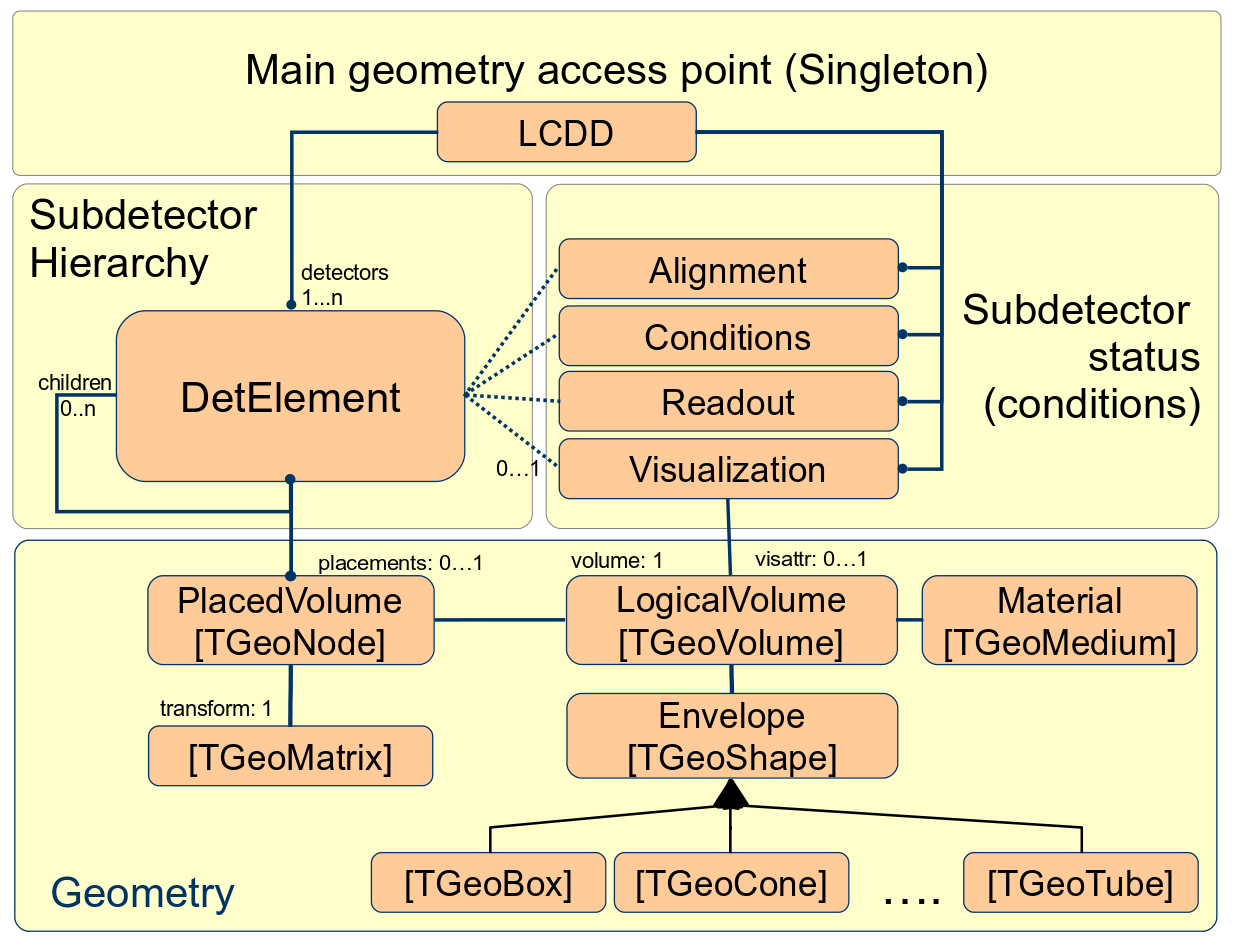
\includegraphics[height=90mm] {DD4hep_classes}
    \caption{Class diagram with the main classes and their relations 
             for the Generic Detector Description Model. The implementing
             ROOT classes are shown in brackets.}
    \label{fig:dd4hep-detector-model}
  \end{center}
\end{figure}
\vspace{-0.1cm}
%=============================================================================
\subsection{Generic Detector Description Model}
\label{subsec:generic-model}
%=============================================================================

\noindent
This is the heart of the DD4hep detector description toolkit. Its purpose is 
to build in memory a model of the detector including its geometrical aspects
as well as structural and functional aspects. The design reuses the elements 
from the ROOT geometry package and extends them in case required functionality 
is not available. Figure~\ref{fig:dd4hep-detector-model} illustrates the main
players and their relationships~\cite{bib:DD4hep}.
Any detector is modeled as a tree of $Detector$ $Elements$, the entity 
central to this design, which is represented in the implementation by 
the $DetElement$ class~\cite{bib:LHCb-geometry}. It offers all
applications a natural entry point to any detector part of the experiment
and represents a complete sub-detector (e.g. TPC), a part of a 
sub-detector (e.g. TPC-Endcap), a detector module or any other convenient 
detector device. 
The main purpose is to give access to the data associated 
to the detector device. For example, if the user writes some TPC reconstruction 
code, accessing the TPC detector element from this code will provide access 
the all TPC geometrical dimensions, the alignment and calibration constants 
and other slow varying conditions such as the gas pressure, end-plate 
temperatures etc. The $Detector$ $Element$ acts as a data concentrator. 
Applications may access the full experiment geometry and all connected data
through a singleton object of type $Detector$, which provides 
management, bookkeeping and ownership to the model instances.

\noindent
The geometry is implemented using the ROOT geometry classes, which are used
directly without unnecessary interfaces to isolate the end-user from the 
actual ROOT based implementation.
\DDA allows client to access, manage and apply alignment parameters or 
smallish changes to the ideal geometry. The mechanism to achieve this 
is described in the following.


%=============================================================================
\begin{figure}[h]
  \begin{center}
    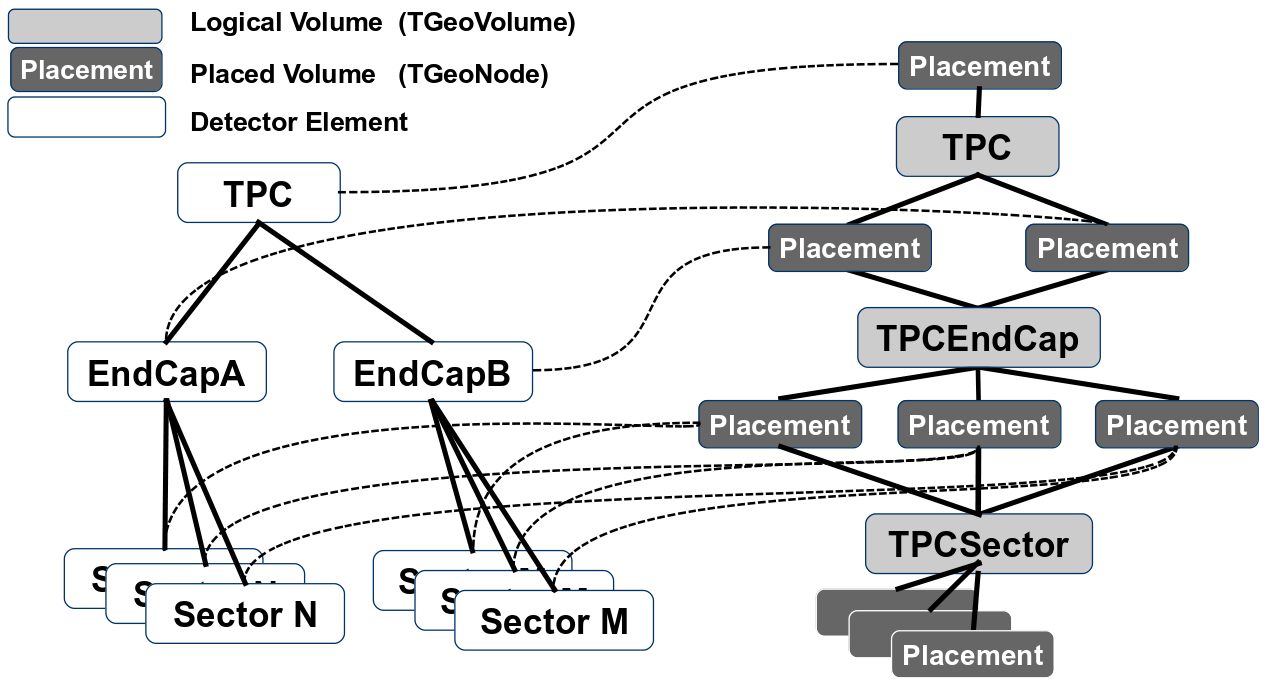
\includegraphics[height=75mm] {DD4hep_detelement_tree}
    \caption{The object diagram of a hypothetical TPC detector showing in
    parallel the $Detector$ $Element$ and the $Geometry$ hierarchy and the 
    relationships between the objects.}
    \label{fig:dd4hep-hierarchies}
  \end{center}
  \vspace{-0.5cm}
\end{figure}


%=============================================================================
\subsection{Detector Element Tree and the Geometry Hierarchy}
\label{subsect:detelement-hierarchy}
%=============================================================================
\noindent
The geometry part of the detector description is delegated to the ROOT classes.
$Logical$ $Volumes$ are the basic objects used in building the geometrical hierarchy. 
A $Logical$ $Volume$ is a shape with its dimensions and consist of a given material. 
They represent unpositioned objects which store all information about 
the placement of possibly embedded volumes. The same
volume can be replicated several times in the geometry. The $Logical$ $Volume$ 
also represents a system of reference with respect to its containing volumes.
The reuse of instances of $Logical$ $Volumes$ for different placements 
optimizes the memory consumption and detailed geometries for complex setups
consisting of millions of volumes may be realized with reasonable amount of memory.
The difficulty is to identify a given positioned volume 
in space and e.g. apply alignment parameters to one of these volumes. 
The relationship between the Detector Element and the placements
is not defined by a single reference to the placement, but the full path 
from the top of the detector geometry model to resolve existing
ambiguities due to the reuse of $Logical$ $Volumes$.
Hence, individual volumes must be identified by their full path from mother 
to daughter starting from the top-level volume. 

\noindent
The tree structure of
$Detector$ $Elements$ is a parallel structure to the geometrical hierarchy.
This structure will probably not be as deep as the geometrical one since 
there would not need to associate detector information at very fine-grain 
level - it is unlikely that every little metallic screw
needs associated detector information such as alignment, conditions, etc.
Though this screw and many other replicas must be described in the geometry 
description since it may be important e.g. for its material contribution 
in the simulation application. Thus, the tree of Detector Elements is
fully degenerate and each detector element object will be placed only 
once in the detector element tree as illustrated for a hypothetical
Time Projection Chamber (TPC) detector in 
Figure~\ref{fig:dd4hep-hierarchies} with an ideal geometry,
where no positioning corrections are applied to neither child. 
It is essential to realize that the geometry tree in an ideal geometry is
degenerate contrary to the tree of detector elements.

\noindent
It should be noted, that alignment parameters may be applied to any volume 
of the ideal geometry. The alignment only affects the actual position of 
a volume it is e.g. irrelevant if the volume is sensitive or not.

%=============================================================================
\begin{figure}[h]
  \begin{center}
    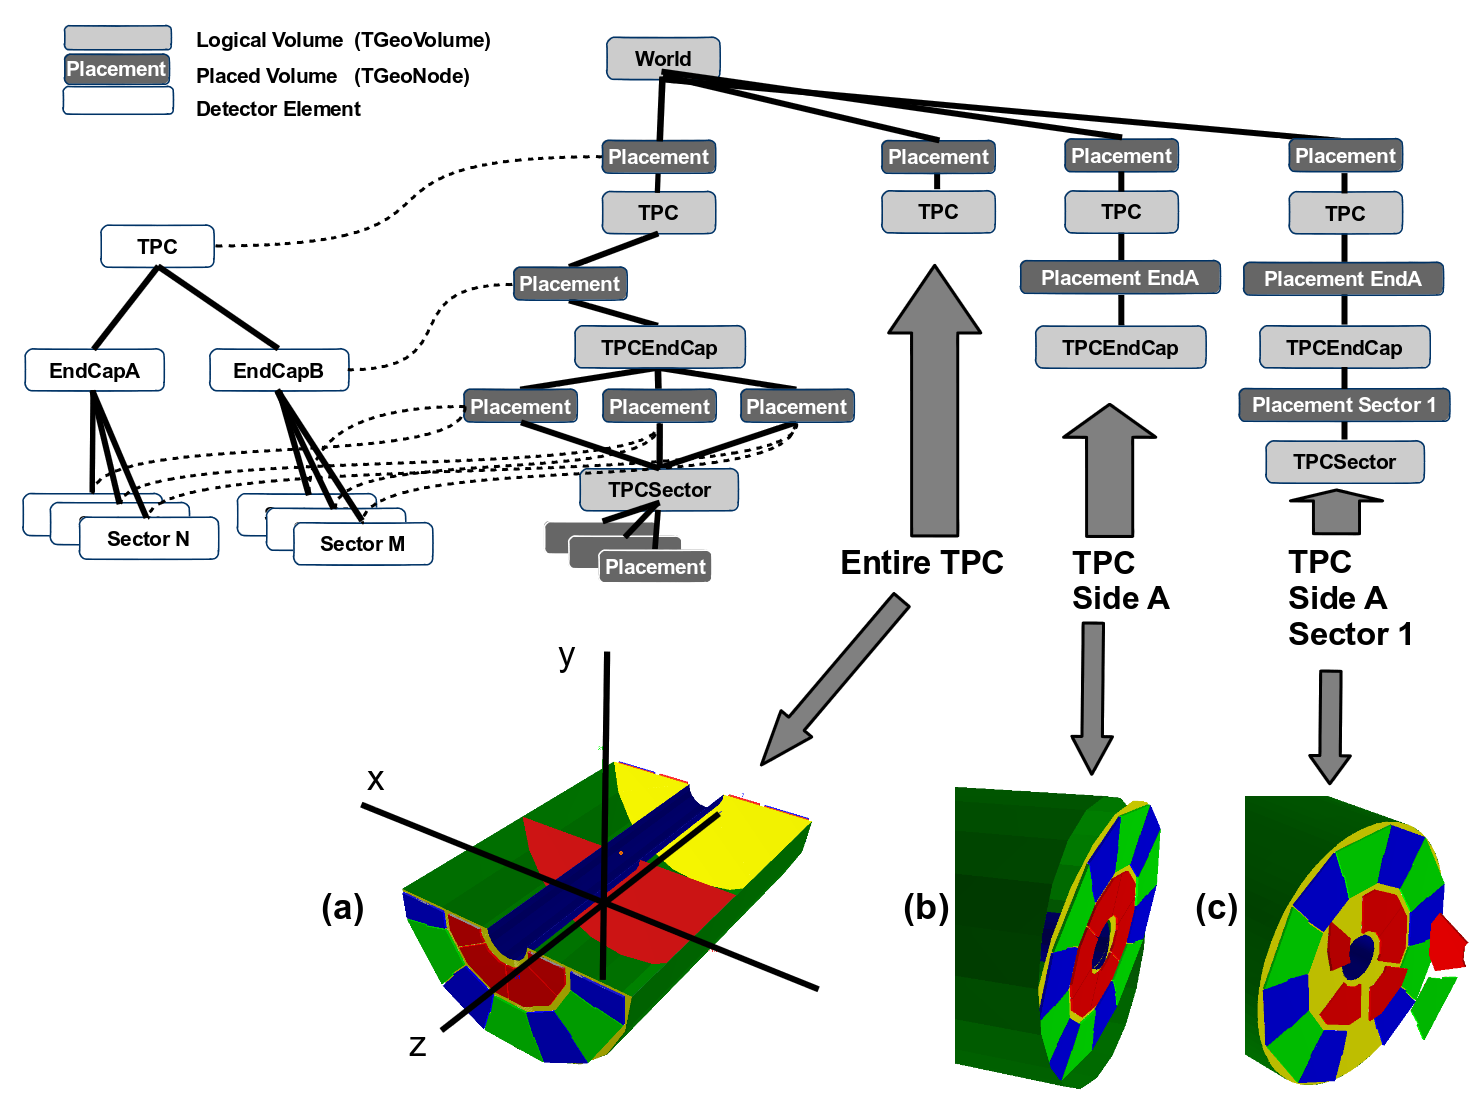
\includegraphics[width=160mm] {DDAlign_detelement_aligned_tree}
    \caption{The object diagram of a hypothetical TPC detector showing in
    parallel the $Detector$ $Element$ and the $Geometry$ hierarchy and examples
    of mispositioned detector parts: (a) mispositioned entire subdetector 
    (translation), (b) mispositioned end-cap (tilt) and (c) mispositioned
    individual sectors within one endcap.}
    \label{fig:dd4hep-aligned-hierarchies}
  \end{center}
\end{figure}

%=============================================================================
\section{Global Alignment}
\label{sect:ddalign-global-aligments}
%=============================================================================
\subsection{Global Alignment of Detector Components}
\label{subsect:ddalign-intro-aligments}
%=============================================================================
\noindent
In this section the backgrounds of the {\it{Global Alignment}} is described.
Alignment parameters never apply in the same way to {\it{all}} placements of the 
same volume in this hierarchy. Hence, to (re-)align a volume in the hierarchy
means to logically lift a full branch of placements from the top volume down to
the element to be (re-)aligned out of this shared hierarchy and apply
a correction matrix to the last node. This procedure is illustrated in 
Figure~\ref{fig:dd4hep-aligned-hierarchies}. Re-alignment of volumes may occur
at any level. In the above example of a TPC this results in the following effects:

\noindent
\begin{itemize}\itemcompact
\item A realignment of the entire subdetector, i.e. the TPC as a whole, 
    would affect consequently move all contained children with respect to the 
    top level coordinate system. An example is shown in 
    Figure~\ref{fig:dd4hep-aligned-hierarchies} (a). A movement of the subdetector
    would affect all transformation between local coordinates of any part of the
    subdetector to the top level coordinate system. Such effects would be visible 
    at all stages of the data processing e.g. when translating signals from 
    particles into global coordinates.
\item A realignment of parts of a subdetector affects only the partial subdetector
    itself and child volumes at lower levels. As in the example, where the entire
    subdetector is moved, here only the sectors on one 
    side of the TPC would be affected
    as shown in Figure~\ref{fig:dd4hep-aligned-hierarchies} (b).
\item In Figure~\ref{fig:dd4hep-aligned-hierarchies} (c) within one 
    end-cap of the TPC
    individual sectors may not be positioned at the ideal location
    (Figure~\ref{fig:dd4hep-aligned-hierarchies} (c) exaggerates: 
    ''flying sectors'' are a rather rare case in reality).
    Finally also the sectors itself could be fragmented and be assemblies of other
    shapes, which are not ideally placed and may need correction.
\end{itemize}
The origin of the volume misplacements may be many-fold:
\begin{itemize}\itemcompact
\item Elements may be weak and assembled parts move due to weak support
    structures.
    This is a common problem e.g. for tracking detectors, where heavy and solid 
    structures dramatically influence the measurement result.
    Misplaced sectors could e.g. be the consequence of a deforming 
    end-cap frame due to the weight of the sectors.
\item Environmental conditions such as the temperature may influence the 
    position or the shape of a volume.
\item Some of the measurement equipment may be moved from a parking position into 
    a data taking position such as the two halves of the LHCb vertex detector. 
    Whereas the position of the sensors on each half are known to a very high 
    precision, the position of the absolute position of the two halves with
    respect to the full experiment may change after each movement.
\end{itemize}
Changes to the volume placement do not only affect sensitive material 
i.e. detector components with an active readout, but also passive material. 
The placement of any volume, passive or active, may be corrected using \DDA. 
The determination of the alignment parameters of passive components however may
be more difficult in the absence of located signals resulting 
e.g. from the traversal of a track.

\noindent
All effects resulting from such causes obviously need to be corrected in order to 
fully explore the capabilities of the detection devices and to minimize 
measurement errors. In general any deviation from the ideal position of a volume
can be described by two elementary transformations:
\begin{itemize}\itemcompact
\item a translation
\item a rotation around a pivot point.
\end{itemize}
giving a full transformation matrix of the form:
\begin{equation}
T = L * P * R * P^{-1}
\end{equation}
where 
\begin{itemize}\itemcompact
\item $T$ is the full transformation in 3D space containing the change to the 
exiting placement transformation. The existing placement is the placement 
transformation of the volume with respect to the mother volume.
\item $L$ is a translation specifying the position change with respect to the 
    mother volume.
\item $P * R * P^{-1}$ describes a rotation around a pivot point specified 
    int he mother volume's coordinate system.
\item $P$ is the translation vector from the mother volumes origin to the 
    pivot point. The concept of a pivot point does not introduce a new 
    set of parameters. Pivot points only help to increase the numerical
    precision.
\end{itemize}
Most of the changes do not require the full set of parameters. Very often 
the changes only require the application of only a translation, only a
rotation or both with a pivot point in the origin. These simplifications 
are supported  in the user interface described in 
Section~\ref{sec:ddalign-user-manual-ddalign-interface}.

%=============================================================================
\begin{figure}[t]
  \begin{center}
    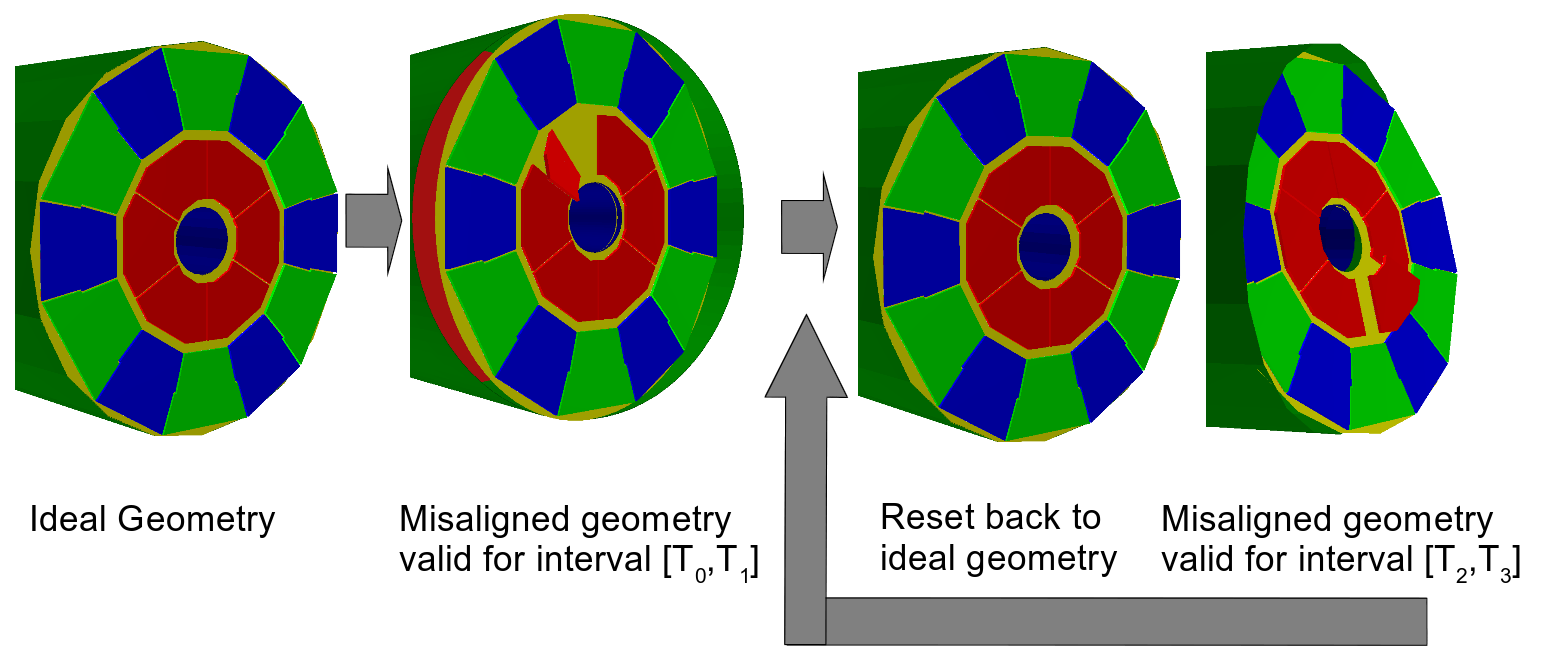
\includegraphics[width=160mm] {DDAlign-iterative-misalignment}
    \caption{The iterative application of alignment parameters as described
    in Section~\ref{subsect:ddalign-intro-iterative-alignments}.
    For each interval of validity 
    ($[T_0,T_1]$, $[T_2,T_3]$, $[T_4,T_5]$, ...)
    a separate set of alignment constants is applied to the ideal geometry.
    The two steps to reset the misaligned geometry back to the ideal
    geometry and
    to re-apply a new set of alignment constants may be executed as 
    often as necessary when processing data from particle collisions.}
    \label{fig:ddalign-aligned-iterative}
  \end{center}
\end{figure}

%=============================================================================
\subsection{Iterative Application of Global Alignments}
\label{subsect:ddalign-intro-iterative-alignments}
%=============================================================================
\noindent
Technically it is possible to apply global alignment procedures iteratively.
This however id {\bf{deprecated}} and violates thread safety for the simple reason
that the {\it{geometry in memory}} is altered. If applied, it is duty of the 
client framework to ensure that during the change of global alignment 
no processing of event data is ongoing.
Hence, the procedure is described here only for completeness:
\begin{enumerate}\itemcompact
\item Create the ideal detector using an ideal geometry.
\item Apply a set of alignment parameters for a given time 
    interval corresponding to the 
    time a set of particle collisions were collected in the experiment.
\item Process the set of collected particle collisions.
\item Reset the misaligned detector to the ideal.
\item Choose new event data input corresponding to another time interval
    and restart at item 2.
\end{enumerate}
Graphically this use case is illustrated in 
Figure~\ref{fig:ddalign-aligned-iterative}. In 
Section~\ref{sec:ddalign-user-manual-ddalign-interface} the implementation 
to realize this use case is described.

%=============================================================================
\subsection{Procedures to Determine Global Alignment Parameters}
\label{subsect:ddalign-intro-determine-alignment-params}
%=============================================================================
\noindent
Typically the determination of alignment parameters requires a starting point
which is not necessarily identical to the ideal position of a 
volume~\cite{bib:chris-parkes-priv-comm}. These volume positions are the result
of a survey measurement or the result of internal position measurements 
of a sub-volume within a sub-detector e.g. on a measurement bench.
In the following we call these parameters {\it{survey parameters}}. 
{\it{Survey parameters}} default to the ideal volume position if not supplied,
alternatively, if set, to the provided position. {\it{Survey parameters}}
are, like the alignment parameters, provided in terms of {\it{changes}} with 
respect to the ideal position and hence may be treated in a similar way.

\noindent 
The survey parameters are accessible to users
through the interface offered by the $DetElement$ objects.

%=============================================================================
\subsection{Simulation of Non-Ideal Detector Geometries}
\label{subsect:ddalign-intro-simulate-misaligned-geometries}
%=============================================================================
\noindent
It is a standard procedure in high energy physics to at least verify 
the measured detector response of a given physics process in particle 
collisions with the expected simulated detector response.
For most purposes the simulation of an ideal detector is certainly is
sufficient - though not describing the full truth. Sometimes however, the
detector geometry must be simulated with a geometry as close to the 
known geometry as possible.

\noindent
The simulation of such a geometry with applied alignment parameters can 
rather easily be realized using using the \DDhep, \DDA and the \DDG frameworks:
\begin{itemize}\itemcompact
\item The ideal geometry is constructed using the standard procedures
    of \DDhep~\cite{bib:DD4hep}.
\item Then the alignment parameters are applied and finally
\item the corrected geometry is translated to $Geant4$~\cite{bib:geant4}
    using the \DDG~\cite{bib:DDG4} package.
    All particle collisions simulated with this translated geometry 
    correspond to the modified geometry including the geometry
    modifications.
\end{itemize}
There is a caveat though: The application of alignment parameters can
easily create volume overlaps, which are highly disliked by the $Geant4$ 
runtime. If the above described procedure is applied, it is highly advised 
to check the resulting geometry for overlaps. Both, 
$ROOT$~\cite{bib:ROOT-tgeo} and $Geant4$~\cite{bib:geant4} offer tools 
to perform such tests.

\noindent
To simulate distorted geometries clients should use the 
$Global$ $Alignment$  interface described in 
section~\ref{sec:ddalign-user-manual-ddalign-global-interface}.

\newpage
%=============================================================================
\subsection{The Global Alignment Interface}
\label{sec:ddalign-user-manual-ddalign-global-interface}
%=============================================================================

\noindent
In this chapter will be documented how to use the $Global$ $Alignment$ 
interface of \DDA. As already mentioned in 
section~\ref{sec:ddalign-user-manual-introduction}, 
this interface allows to alter the layout of the 
geometry in memory. Use cases are e.g. the simulation of 
non-ideal geometries.

\noindent
Global alignment can be applied to detector elements using a specialized
interface {\it{GlobalDetectorAlignment}}~\footnote{See the header file
$DDAlign/GlobalDetectorAlignment.h$ for details.}. This interface 
provides the API to apply global changes to the geometry provided
the presence of alignment parameters as shown in the following 
code snippet:

\begin{code}
  /// First install the global alignment cache to build proper transactions
  Detector& detector = ...;
  GlobalAlignmentCache* cache = GlobalAlignmentCache::install(detector);
  
  /// Now create the transaction context. There may only be one context present
  GlobalAlignmentStack::create();
  GlobalAlignmentStack& stack = GlobalAlignmentStack::get();

  /// Now we can push any number of global alignment entries to the stack:
  DetElement        elt       = ...detector element containing the volume to be re-aligned ...;
  string            placement = "/full/path/to/the/volume/to/be/realigned";  
  Alignments::Delta delta     = ...;
  double            ovl       = allowed_overlap_in cm; // e.g. 0.001;

  // Create the new stack entry and insert it to the stack
  dd4hep_ptr<StackEntry> entry(new StackEntry(elt,placement,delta,ovl));
  stack->insert(entry);

  /// Finally we commit the stacked entries and release the stack.
  cache->commit(stack);
  GlobalAlignmentStack::get().release();
\end{code}

\noindent
{\bf{Explanation:}} \\
\begin{tabular} {l||p{0cm}}
\docline{Line}{}
\docline{3}{Install the $GlobalAlignmentCache$. Required to be done
once. The object is registered to the $Detector$ instance and kept there.}
\docline{3-8}{The fact that the classes $GlobalAlignmentCache$ and 
$GlobalAlignmentStack$ are singletons is not a fundamental issue.
However, we want to call the XML parser (or other database sources)
iteratively and currently cannot chain a context (stack).}
\docline{16-21}{The created stacked entries are automatically released 
once the transaction is committed.}
\end{tabular}

\noindent
Please note, that this interface normally is not directly invoked
by users, but rather called by plugin mechanisms as the one described below
capable of reading the global misalignments from XML.

\noindent
%=============================================================================
\subsubsection{Loading Global Geometrical Imperfections from XML}
\label{sec:ddalign-user-manual-global-misalignment-manip-xml}
%=============================================================================
\noindent
In this section we describe how to load global geometry 
imperfections and to apply them
to an existing geometry. Loading the XML file is done automatically using the 
standard XML loader plugin provided by \DDhep. This mechanism is favoured and 
much simpler than programming the global misalignment directly.
This plugin is interfaced to 
the {\tt Detector} instance and invoked from code as follows:
\begin{code}
    Detector& detector = ....;
    detector.fromXML("file:AlepTPC_alignment.xml");
\end{code}
To fully exploit the capabilities it is important to understand the interpreted 
structure of the XML file being processed. At the top level of the primary 
input file (i.e. the file given to the XML processor) the following structure 
is expected:
\begin{code}
<global_alignment>
  <!-- Open the alignment transaction  -->
  <open_transaction/>
  <subdetectors>         <!-- Container with the list of subdetectors to be processed. -->
    <detelement path="TPC" reset="true" reset_children="true">
      <!-- Move the entire TPC in the world volume                                     -->
      <position="" x="30"   y="30"  z="80"/>

      <!-- Now add daughter detector elements                                          -->

      <!-- Twist a bit the entire endcap by rotating it around the x and the y axis    -->
      <detelement path="/world/TPC/TPC_SideA" check_overlaps="false">
        <position x="0"   y="0"  z="0"/>
        <rotation x="-0.2" y="-0.2"  z="0"/>
        <!-- Apply corrections of type Translation*Rotation to a single sector           
        <detelement path="TPC_SideA_sector02" check_overlaps="true">
          <position x="0"   y="0"   z="0"/>
          <rotation x="0.5" y="0.1" z="0.2"/>     
        </detelement>
      </detelement>

      <!-- And the full shooting match of transformations for this sector              -->
      <detelement path="TPC_SideA/TPC_SideA_sector03" check_overlaps="true">
        <position x="0" y="0"    z="290.0*mm"/>
        <rotation x="0" y="pi/2" z="0"/>     
        <pivot    x="0" y="0"    z="100"/>     
      </detelement>

      ....

      <!-- Include alignment files to be processed in the context of the "TPC" DetElement
      <include ref="file-name"/>

    </detElement>            
  </subdetectors>

  <!-- Include alignment files to be processed at the top level context               -->
  <include ref="file-name"/>

  <!-- Close the alignment transaction  -->
  <close_transaction/>
</global_alignment>
\end{code}

\noindent
The structure of the alignment file explained quickly:

\begin{tabular} {l||p{0cm}}
\docline{Line}{}
\docline{1}{The {\tt root} tag for the primary alignment file is {\tt <alignment/>}.
    The primary tag name is mandatory and actually is used to invoke the correct interpreter.}
\docline{2,41}{Trigger the alignment transaction by specifying the transaction tags in 
        the main XML file.}
\docline{4}{Definition of the set of {\tt subdetectors} to be processed. A valid alias for this
        directive is {\tt detelements}.}
\docline{5}{The first subdetector: {\tt TPC}. The subdetector tag is {\tt detelement}
        Each {\tt detelement} may recursively contain other {\tt detelement} tags.
        as they were defined in the {\tt DetElement} hierarchy.
        Internal {\tt detelement} elements are processed in the context of the outer
        element i.e. paths may be specified relative to the parent or as absolute paths
        with respect to the world (starting with a '/').}
\docline{7}{Global movement of the TPC}
\docline{12-20}{Realignment entry for the TPC endcap A named {\tt TPC\_SideA}}
\docline{16-19}{Realignment entry for sector named {\tt TPC\_SideA\_sector02} of the TPC endcap A.
    Here the sector is specified directly as a daughter of the endcap. The name 
    of the {\tt DetElement} is relative to the parent.}
\docline{23-27}{Realignment entry for sector named {\tt TPC\_SideA\_sector03} of the TPC endcap A
        containing a full transformation: $Translation * Pivot * Rotation * Pivot^{-1}$}
\docline{32}{Optionally {\tt detelement} elements may include other alignment files specifying
        lower volume levels. These files are interpreted in the context of the calling 
        detector element. }
\docline{38}{Optionally the subdetector alignment constants may be fragmented 
        into several files,   which can be loaded using the {\tt include} 
        directive. Each file could for example describe one single detector.}
\end{tabular}

\vspace{0.5cm}
\noindent
The specification of any transformation element is optional:
\begin{itemize}\itemcompact
\item The absence of a translation implies the origin (0,0,0)
\item The absence of a pivot point implies the origin (0,0,0)
\item The absence of a rotation implies the identity rotation.
    Any supplied pivot point in this case is ignored.
\end{itemize}
The absence of a transformation element is absolutely legal and does not
issue any warning or error.

\noindent
All transformations describe the change of placement with respect to the 
coordinate system of the closest mother-volume in the volume hierarchy,
i.e. translations, rotations and pivot points are local to the 
mother coordinate system.

\noindent
Included files may directly start with the {\tt root} tags {\tt subdetectors}, 
{\tt detelements} or {\tt detelement} and may recursively include other
files. Except for the top level these files are processed in the calling context.
The result of this procedure is shown in Figure~\ref{fig:dd4hep-aligned-hierarchies}.

%=============================================================================
\begin{figure}[h]
  \begin{center}
    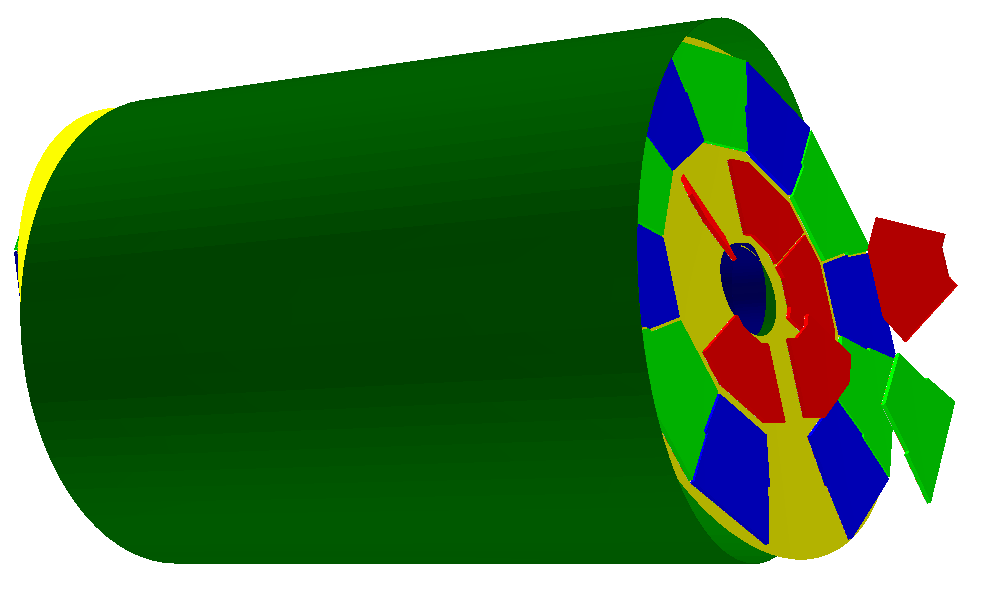
\includegraphics[width=160mm] {DDAlign-misaligned-TPC}
    \caption{The ALEPH TPC after the import of the alignment file.
    Note, that the geometry in $memory$ changed. The original
    geometry description is no longer present.
    }
    \label{fig:dd4hep-aligned-hierarchies}
  \end{center}
\end{figure}


\noindent
%=============================================================================
\subsubsection{Export Geometrical Imperfections to XML}
\label{sec:ddalign-user-misalignment-expotr-xml}
%=============================================================================
\noindent
In this section we describe how to export geometry imperfections to an XML file.
A small helper class {\tt AlignmentWriter} achieves this task as shown in 
the snippet:
\begin{code}
  Detector&  detector = ....;
  DetElement top = detector.world();
  if ( top.isValid() )   {
    AlignmentWriter wr(detector);
    return wr.write(top,output,enable\_transactions);
  }
\end{code}
This code will dump all alignment constants contained in the {\tt DetElement}
hierarchy of {\tt top} to the output file {\tt output}. The optional argument
{\tt enable\_transactions} (default: true) will add the tags 
{\tt <open\_transaction/>} and {\tt <close\_transaction/>} to the output 
file. The output file conforms to the specifications described in 
Section~\ref{sec:ddalign-user-manual-misalignment-manip-xml} and may later
be imported by another process.

\noindent
{\bf{FIXME: This chapter sort of still has to be written/completed!!!!}}

\newpage

\section{Up to here the manual should be pretty much correct.\\
Everything below is at least questionable.}

%=============================================================================
\section{Local Alignment}
\label{sect:ddalign-local-aligments}
%=============================================================================
bla bla bla

%%%% Here we are now.






%%%%%%%%%%%%%%%%%%%%%%%%%%%%%%%%%%%%%%%%%%%%%%%%%%%%%%%%%%%%%%%%%%%%%%%%%%%%%%%


\noindent
Generally such a behavior can be achieved in two ways. The usage strongly depends
on the use-case required by the client:
\begin{enumerate}
\item either the ideal geometry in memory is changed directly to 
      reflect the  measured geometry. This approach has the 
      disadvantage, that all measurement points on a daughter 
      volume can only be transformed to the global coordinate
      system using one single transformation. Time-dependent changes of 
      these transformations cannot be modeled. Hence, for multi-threaded
      systems this approach is of limited use. However, this is the 
      perfect approach to simulate distorted geometries. This approach 
      is naturally supported by the ROOT geometry toolkit.
\item The second possibility is to not modify the ideal geometry in memory,
      but to provide instead transformations to move measured coordinates 
      to their correct place in space. This approach allows to keep 
      several - also time-dependent - transformations in memory. 
      Ideal to support multi-threaded data processing frameworks, 
      which become more and more popular.
\end{enumerate}

\noindent
\DDA supports both possibilities as will be described in the following sections.



\vspace{3cm}

\newpage
%=============================================================================
\section{The Local Alignment Interface}
\label{sec:ddalign-user-manual-ddalign-interface}
%=============================================================================

\noindent
\DDA implements a machinery to apply and access the alignment parameters
describing the difference between an ideal detector given by an ideal geometry
and the geometry of the actually built assembly in real life.
To ease its usage for the clients and to shield clients from the 
internals when actually dealing with realigned geometries, a set of 
helper classes was designed. The access to the alignment parameters 
in read-only mode was separated from the import or export thereof.

\noindent
As a basic concept within \DDhep any {\it{sizable}} detector component
can be realigned. {\it{Sizable}} as a rule of thumb is anything, which 
is manufactured as an individual piece and which you may ''hold in your hands''.
Such objects are also described by a $detector$ $element$ of type {\tt DetElement}.
An example is e.g. a single silicon wafer of a tracking device or the entire
tracking detector itself.
The access to the alignment parameters is possible from each {\tt DetElement}
instance as described in Section~\ref{sec:ddalign-user-manual-misalignment-access}.
The interface assumes ''planar'' alignment parameters i.e. the shape of 
a given volume does not change~\footnote{This is a restriction to the 
possibilities provided by the ROOT implementation~\cite{bib:ROOT-tgeo}
based on experience~\cite{bib:chris-parkes-priv-comm}.
If at a later time the need arises the provided alignment interface may 
be extended to support shape changes.}.

\noindent
As mentioned earlier, in the local alignment \DDA allowed to retrieve 
time dependent alignment parameters and transformations. This time
dependency was relatively easy achieved by re-using the conditions 
mechanism from \DDC. In this spirit Alignment transformations are 
practically no different from conditions like temperatures, pressures etc.
To access the $alignment$ $conditions$ clearly not only some 
identifier must be provided, but also a $interval$ $of$ $validity$,
which defines from which point in the past to which point in the future
the required alignment constants may be applied.

\noindent
Please be aware that the extensive use of misalignments is highly memory
consuming.

\noindent
%=============================================================================
\subsection{Access to Alignment Parameters from the Detector Element}
\label{sec:ddalign-user-manual-misalignment-access}
%=============================================================================

\noindent
The $DetAlign$ class as shown in Figure~\ref{fig:dd4hep-detector-model}
gives the user access to the alignment structure of type $Alignment$ as 
illustrated in the following example:
\begin{code}
    ConditionsSlice slice = ...  // Prepared slice containing all conditions
    DetElement wafer_det  = ...  // Valid handle to a detector element
    DetAlign   wafer = wafer_det;
    Alignment  wafer_alignment = wafer.get();
    if ( wafer_alignment.isValid() )  {
        // This wafer's placement differs from the ideal geometry when
        // alignment parameters are present.
        
        // Access the misalignment transformation with respect to the parent volume:
        Transform3D tr = wafer_alignment.toMotherDelta();
    }
\end{code}
The access to details of an invalid alignment object results in a runtime 
exception. The following calls allow clients to access alignment information
from the $DetElement$ structure:
\begin{code}
      /// Access to the actual alignment information
      Alignment alignment() const;

      /// Access to the survey alignment information
      Alignment surveyAlignment() const;
\end{code}
The call to $alignment()$ return the parameters $applied$ to the the existing
ideal geometry. The call $surveyAlignment()$ returns optional constants used 
to perform numerical calculations as described in 
section~\ref{subsect:ddalign-intro-determine-alignment-params}.

\noindent
All functionality of the DetElement, which depends on applied alignment parameters
are automatically updated in the event of changes. These are typically the geometry 
transformations with respect to the mother- and the world volume:
\begin{code}
      /// Create cached matrix to transform to world coordinates
      const TGeoHMatrix& worldTransformation() const;

      /// Create cached matrix to transform to parent coordinates
      const TGeoHMatrix& parentTransformation() const;
 
      /// Transformation from local coordinates of the placed volume to the world system
      bool localToWorld(const Position& local, Position& global) const;

      /// Transformation from local coordinates of the placed volume to the parent system
      bool localToParent(const Position& local, Position& parent) const;

      /// Transformation from world coordinates of the local placed volume coordinates
      bool worldToLocal(const Position& global, Position& local) const;

      /// Transformation from world coordinates of the local placed volume coordinates
      bool parentToLocal(const Position& parent, Position& local) const;
\end{code}
it is worth noting that the update of cached information is performed by the $DetElement$ 
objects, other user defined cached information is {\bf{not}} updated. To update 
user caches it is mandatory to provide a user defined update callback to the $DetElement$:
\begin{code}
    template <typename Q, typename T> 
    void callAtUpdate(unsigned int type, Q* pointer, 
                      void (T::*pmf)(unsigned long typ, DetElement& det, void* opt_par)) const;
\end{code}

\noindent
The interface of the $Alignment$ structure to access detector 
alignment parameters is as follows (see also the corresponding header file DD4hep/Alignment.h):
\begin{code}
      /// Number of nodes in this branch (=depth of the placement hierarchy from the top level volume)
      int numNodes() const;
      
      /// Access the placement of this node
      PlacedVolume placement()   const;

      /// Access the placement of the mother of this node
      PlacedVolume motherPlacement(int level_up = 1)   const;

      /// Access the placement of a node in the chain of placements for this branch
      PlacedVolume nodePlacement(int level=-1)   const;

      /// Access the currently applied alignment/placement matrix with respect to the world
      Transform3D toGlobal(int level=-1) const;

      /// Transform a point from local coordinates of a given level to global coordinates
      Position toGlobal(const Position& localPoint, int level=-1) const;

      /// Transform a point from global coordinates to local coordinates of a given level
      Position globalToLocal(const Position& globalPoint, int level=-1) const;

      /// Access the currently applied alignment/placement matrix with respect to mother volume
      Transform3D toMother(int level=-1) const;

      /// Access the currently applied alignment/placement matrix (mother to daughter)
      Transform3D nominal() const;

      /// Access the currently applied correction matrix (delta) (mother to daughter)
      Transform3D delta() const;

      /// Access the inverse of the currently applied correction matrix (delta) (mother to daughter)
      Transform3D invDelta() const;
\end{code}
\begin{itemize}\itemcompact
\item The calls in line 3-8 allow access to the relative position of the $nth.$ element
    in the alignment stack with respect to its next level parent. 
    Element $numNodes()-1$ denotes the lowest level and element $0$ is the world 
    volume. The default argument $(-1)$ addresses the lowest placement in the hierarchy.
\item Calls in line 9-12 allow to access/execute transformations from a given level
    in the placement hierarchy to coordinates in the top level volume (world).
\item The call in line 14 allows to transform a global coordinate to the local coordinate
    system in a given level of the hierarchy.
\item The call $toMother$ in line 16 returns the local transformation of the node at
    a given level to the mother's coordinate system.
\item The calls in line 17-20 give access to the nominal placement matrix of the realigned
    node with respect to the parent volume and the changes thereof.
\end{itemize}
Besides these convenience calls the full interface to the class {\tt TGeoPhysicalNode}, 
which implements in the ROOT geometry package alignment changes, is accessible 
from the $Alignment$ handle using the overloaded $operator->()$.
Further documentation is available directly from the \tgeo{TGeoPhysicalNode}{ROOT site}.

\noindent
%=============================================================================
\subsection{Manipulation of Alignment Parameters}
\label{sec:ddalign-user-manual-misalignment-manip}
%=============================================================================
There are multiple possibilities to apply alignment parameters:
\begin{itemize}\itemcompact
\item The pedestrian way ''by hand'' using C++ as described in 
    Subsection~\ref{sec:ddalign-user-manual-misalignment-manip-cxx}
\item Loading a whole set of misalignment constants from XML, the ''poor man's'' database.
    This mechanism is described in
    Subsection~\ref{sec:ddalign-user-manual-misalignment-manip-xml}
\item Loading a whole set of misalignment constants from a database.
    This possibility depends heavily on the database and its schema used.
    A typical use case is to load misalignment constants depending on the
    experiment conditions at the time the event data were collected.
    \DDA does not provide an implementation.
    This possibility here is only mentioned for completeness and will be subject 
    to further developments to support conditions in \DDhep. 
\end{itemize}

\noindent
%=============================================================================
\subsubsection{Manipulation of Alignment Parameters for Pedestrians using C++}
\label{sec:ddalign-user-manual-misalignment-manip-cxx}
%=============================================================================
\noindent
In this section we describe how to apply geometry imperfections to an existing 
detector geometry in memory using {\tt C++}. To apply misalignment to an existing
geometry two classes are collaborating, the {\tt AlignmentCache} attached to
the geometry container {\tt Detector} and a temporary structure the {\tt AlignmentStack}.
The {\tt AlignmentCache} allows to access all existing alignment entries 
based on their subdetector.
The {\tt AlignmentStack} may exist in exactly one instance and is used to
insert a consistent set of alignment entries. Consistency is important because
changes may occur at any hierarchical level and internal transformation caches
of the ROOT geometry package must be revalidated for all branches containing
a higher level node.
{\bf For this reason it is highly advisable to apply realignment constants 
for a complete subdetector.}
Note that this restriction is not imposed, in principle a consistent set 
of misalignments may be applied at any level of the geometry hierarchy.

\noindent
Though the application of alignment is much simpler using XML files, the following
description should give an insight on the mechanisms used behind the scene and
to understand the concept.

\noindent
Any manipulations are transaction based must be embraced by the following two calls
opening and closing a transaction:
\begin{code}
// Required include file(s)
#include "DDAlign/AlignmentCache.h"

    Detector& detector = ....;
    AlignmentCache* cache = detector.extension<Geometry::AlignmentCache>();

    // First things first: open the transaction.
    cache->openTransaction();

    // Prepare the entry containing the alignment data
    AlignmentStack::StackEntry* entry =  .....;
    //.... and add the element to the AlignmentStack .....
    AlignmentStack::insert(entry);

    // Finally close the transaction. At this moment the changes are applied.
    cache->closeTransaction();
\end{code}
In the following we describe the mechanism to create and prepare the 
{\tt StackEntry} instances of the above code snippet. The calls to open and close
the alignment transaction do not have to be in the same code fragment where also
the alignment entries are prepared. However, all changes are only applied when 
the transaction is closed. The alignment entries do not necessarily have to 
be prepared in the sequence of the hierarchy they should be applied, internally
the entries are re-ordered and follow the geometry hierarchy top to bottom
i.e. mother volumes are always re-aligned {\it\bf before} the daughters 
are re-aligned.

\noindent
The {\tt StackEntry} instances carry all information to apply the re-alignment 
of a given volume. This information contains:
\begin{itemize}\itemcompact
\item The transformation matrix describing the positional change of the volume
    with respect to its mother volume.
\item The placement path of the volume to be realigned.
\item A flag to reset the volume to its ideal position {\it\bf before} the 
    change is applied.
\item A flag to also reset all daughter volumes to their 
    ideal position {\it\bf before} the change is applied.
\item A flag to check for overlaps after the application of the change and
\item the actual precision used to perform this check.
\end{itemize}

\noindent
The {\tt ROOT::Math} library provides several ways to construct the required
3D transformation as described in Section~\ref{subsect:ddalign-intro-aligments}:
\begin{code}
// Required include file(s)
#include "DD4hep/Objects.h"

    Position      trans(x_translation, y_translation, z_translation);
    RotationZYX   rot  (z_angle, y_angle, x_angle);
    Translation3D pivot(x_pivot, y_pivot, z_pivot);

    Transform3D trafo;
    /// Construct a 3D transformation for a translation and a rotation around a pivot point:
    trafo = Transform3D(Translation3D(trans)*pivot*rot*(pivot.Inverse()));

    /// Construct a 3D transformation for a translation and a rotation around the origin
    trafo = Transform3D(rot,pos);

    /// Construct a 3D transformation for a rotation around a pivot point
    trafo = Transform3D(piv*rot*(piv.Inverse()));

    /// Construct a 3D transformation for a rotation around the origin
    trafo = Transform3D(rot);

    /// Construct a 3D transformation for simple translation
    trafo = Transform3D(pos);

\end{code}

\noindent
The following code snippet shows how to extract this information from the
{\tt DetElement} and prepare such a {\tt StackEntry} instance:
\begin{code}
// Required include file(s)
#include "DDAlign/AlignmentStack.h"

    // Prepare the entry containing the alignment data
    typedef AlignmentStack::StackEntry Entry;
    /// Detector element to be realigned
    DetElement element = ...;
    /// The transformation describing the relative change with respect to the mother volume
    Transform3D trafo = ...;
    /// Instantiate a new alignment entry
    Entry* entry = new Entry(element);
    entry->setTransformation(trafo)                         // Apply the transformation matrix
        .applyReset(/* argument default: true */)           // Set the reset flag
        .applyResetChildren(/* argument default: true */)   // Set the daughter reset flag
        .checkOverlaps(/* argument default: true */)        // Set flag to check overlaps
        .overlapPrecision(0.001/mm);                        // With this precision in mm

    /// Now add the entry to the alignment stack:
    AlignmentStack::insert(entry);
\end{code}
The constructor will automatically determine the volumes placement path
from the {\tt DetElement}. Then the transformation is applied and the flags
to reset the volume, its children and to trigger the overlap checks with 
the given precision.

\noindent
When passing the entry to the {\tt AlignmentStack} the {\tt AlignmentStack}
takes ownership and subsequently the entry is deleted after being applied to
the geometry. For further shortcuts in the calling sequence please consult the
{\tt AlignmentStack} header file.



\newpage
%=============================================================================
\begin{thebibliography}{9}
\bibitem{bib:DD4hep} M. Frank et al, "DD4hep: A Detector Description Toolkit 
                for High Energy Physics Experiments",
                International Conference on Computing in High Energy and Nuclear Physics  
                (CHEP 2013), \\
                Amsterdam, Netherlands, 2013, proceedings.

\bibitem{bib:LHCb-geometry} S. Ponce et al., 
                "Detector Description Framework in LHCb", 
                International Conference on Computing in High Energy and Nuclear Physics  (CHEP 2003), 
                La Jolla, CA, 2003, proceedings. 
\bibitem{bib:chris-parkes-priv-comm} C. Parkes, private communications.
\bibitem{bib:DDG4} M.Frank, "DDG4 - A Simulation Toolkit for High Energy 
                Physics Experiments using Geant4 \\
                and the DD4hep Geometry Description".
\bibitem{bib:ROOT-tgeo} R.Brun, A.Gheata, M.Gheata, "The ROOT geometry package",\\
                    Nuclear Instruments and Methods {\bf{A}} 502 (2003) 676-680.
\bibitem{bib:geant4}  S. Agostinelli et al., 
                   "Geant4 - A Simulation Toolkit", \\
                    Nuclear Instruments and Methods {\bf{A}} 506 (2003) 250-303.
\bibitem{bib:DDCond} M.Frank, "DDCond -- Conditions Support for the DD4hep Geometry Description Toolkit".

\end{thebibliography}
%=============================================================================
\end{document}
